\chapter[Ferramentas Utilizadas]{Ferramentas Utilizadas}
\label{chap:ferramentas}
	
	Nesta seção seção serão apresentadas as descrições das ferramentas utilizadas para produção do projeto, bem como suas funções durante o processo de desenvolvimento das atividades.

	\section[Fluid Ui]{\emph{Fluid Ui}}
	\label{sec:ferramentas_fluidUI}

		A ferramenta usada para criação dos protótipos de baixa fidelidade foi o Fluid Ui. O Fluid Ui é uma ferramenta web para criação de protótipos mobile de baixa fidelidade que disponibiliza três versões pagas e uma free, o aplicativo interage dinamicamente com o usuário na criação simples de prototipos elegantes e robostos. No entanto, a versão free possui diversas limitições de funções tais como a importação de protótipos criados, a criação de mais de 10 telas ou a criação de mais de 2 projetos. Mas, mesmo com a limitações impostas na versão free, foi possível criar de forma efetiva os protótipos. \cite{fluid}

		\begin{figure}[h]
			\centering
			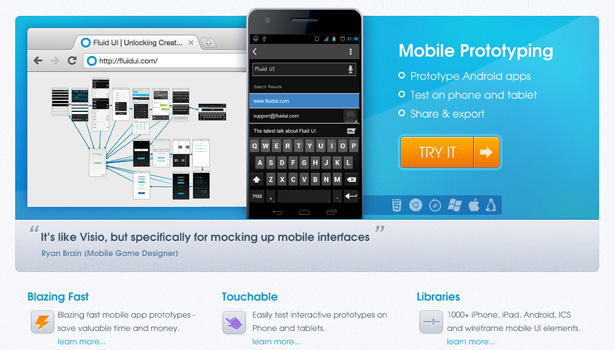
\includegraphics[scale=0.6]{fluid_ui}
			\caption[Fluid UI]{Fluid UI.}
			\label{fig:fluid_ui}
		\end{figure}

	\section[BitStrips]{\emph{BitStrips}}
	\label{sec:ferramentas_bitStrips}

		A ferramenta usada para criar o story board foi o BitStrips. Bitstrips.com é um web site onde você cria quadrinhos gratuitamente, de forma simples, mas com muitos recursos. O Bitstrips é um site sem fins lucrativos criados pela Core Matrix para criação, edição e publicação de histórias em quadrinhos, as famosas "comics", online. \cite{bit}

		\begin{figure}[h]
			\centering
			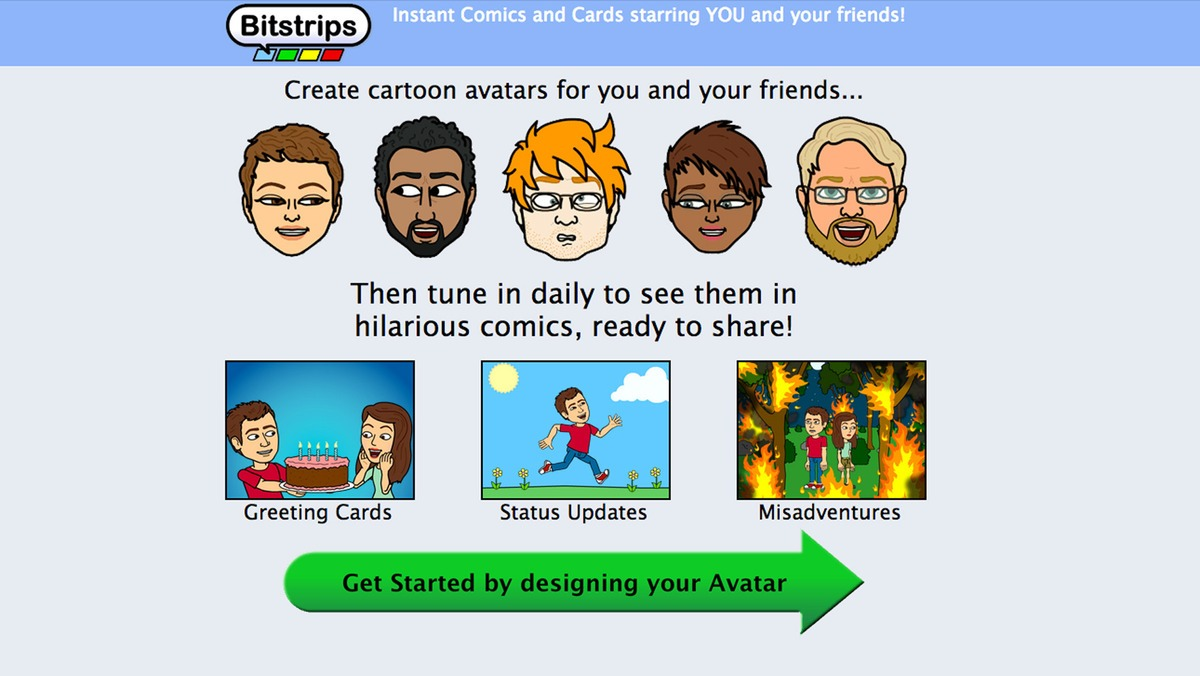
\includegraphics[scale=0.25]{bit_strips}
			\caption[BitStrips]{BitStrips.}
			\label{fig:bit_strips}
		\end{figure}

	\section[Justinmind]{\emph{Justinmind}}
	\label{sec:ferramentas_bitStrips}

		A ferramenta usada para criação dos protótipos de alta fidelidade foi o Justinmind. O Justinmind Prototyper oferece uma excelente solução de design para criação de protótipos para aplicativos, sites, produtos ricos em recursos móveis da web e/ou aplicações empresariais. Além disso, possui uma vasta coleção de bibliotecas de widgets pré-concebidos para começar a criação de protótipos permitindo criar wireframes interativos com interações, animações e até mesmo dados sem ter que se preocupar com codificação. \cite{just}

		\begin{figure}[h]
			\centering
			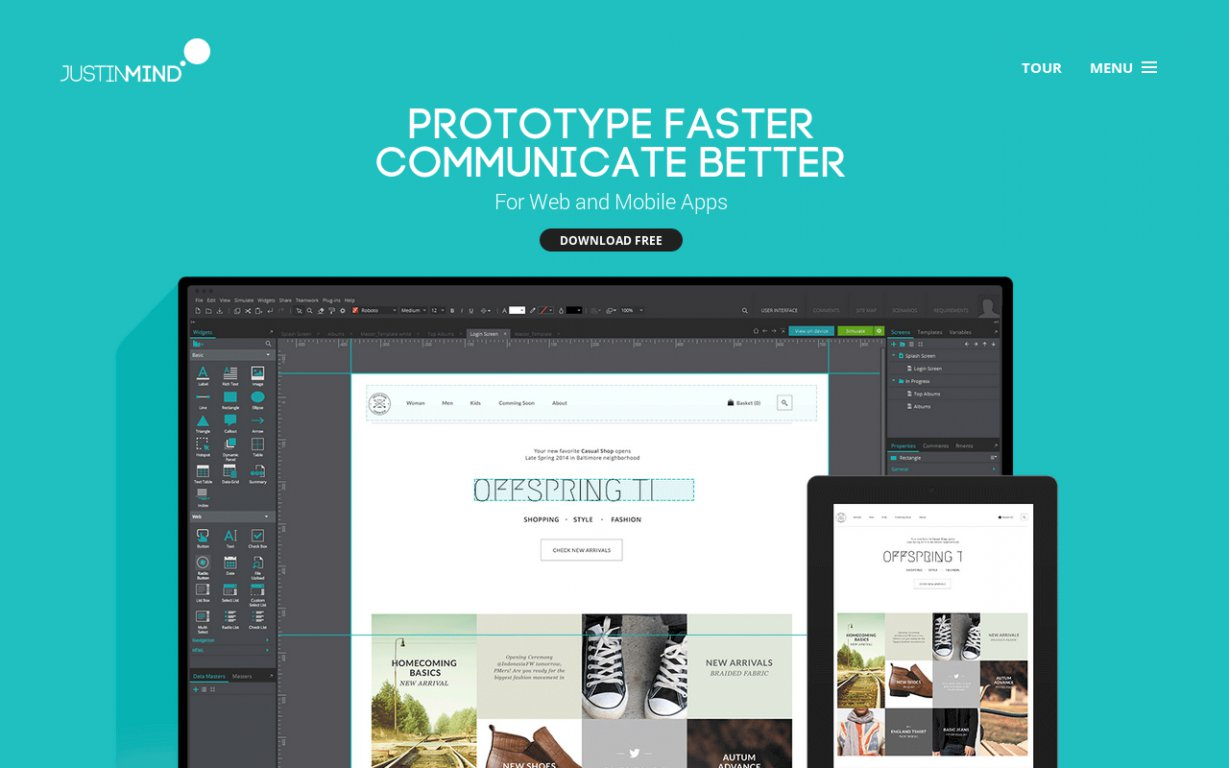
\includegraphics[scale=0.25]{just}
			\caption[Justinmind]{Justinmind.}
			\label{fig:just}
		\end{figure}